\documentclass{bioinfo}
\copyrightyear{2016}
\pubyear{2016}

\usepackage{amsmath}
\usepackage{graphicx}
\usepackage{natbib}

\bibliographystyle{apalike}


\begin{document}
\firstpage{1}

%\title[Evaluating small variant calling]{New benchmark data set provides more accurate estimate of small variant calling error rate}
\title[Evaluating small variant calling]{New benchmark data set for accurate variant calling evaluation}

\author[Li et al]{Heng Li\,$^{1,*}$, Jonathan M Bloom\,$^1$, Yossi Farjoun\,$^1$, Mark
  Fleharty\,$^1$, Laura Gauthier\,$^1$, Benjamin Neale\,$^{1,2,*}$ and Daniel
  MacArthur\,$^{1,2,}$\footnote{to whom correspondence should be addressed}}

\address{$^1$Broad Institute of Harvard and MIT, Cambridge, MA 02142, USA\\
$^2$Analytic and Translational Genetics Unit, Massachusetts General Hospital, Boston, MA 02114, USA}

\maketitle

\begin{abstract}

Constructed from the consensus of multiple variant callers based on short-read
data, existing benchmark data sets for evaluating the variant calling accuracy
are biased towards easy regions accessible by known algorithms.  We derived a
new benchmark data set from the \emph{de novo} PacBio assemblies of two human
cell lines that are homozygous across the whole genome. It provides a more
accurate and less biased estimate of the error rate of small variant calls in a
realistic context.

\end{abstract}

Calling genomic sequence variations from resequencing data plays an important
role in medical and population genetics, and has become an active research area
since the advent of the high-throughput sequencing. Many methods have been
developed for calling single-nucleotide polymorphisms (SNPs) and short
insertions/deletions (INDELs) primarily from short-read data. To measure the
accuracy of these methods and ultimately to make accurate variant calls, we
typically run a variant calling pipeline on benchmark data sets where the true
variant calls are known. The most widely used benchmark data sets include
Genome In A Bottle (GIAB;~\citealp{Zook:2014ab}) and Platinum Genome
(PlatGen;~\citealp{Eberle055541}) for sample NA12878. Both of them come with a set of high-quality
variants and a set of confident regions where non-variant sites are deemed to
be identical to the reference genome. They were constructed from the consensus
of multiple short-read variant callers, with consideration of pedigree
information or structural variations (SVs) found with long-read technologies. A major
concern with GIAB and PlatGen is that the sequencing technologies and the
variant calling algorithms used to construct the data sets are the same as the
ones for testing. This strong correlation leads to biases in two subtle ways.
First, variant calling with short reads is intrinsically difficult in regions
with moderately diverged repeats and segmental duplications.  We have to exclude
such regions from the confident regions as the consensus calls are often
ambiguous. This biases GIAB and PlatGen towards easy genomic regions. In fact,
both benchmark data sets conclude competent variant callers make an error every
5 million bases (Figure~\ref{fig:fig1}a), while other works suggest we can only
achieve an error rate one per 100--200 thousand bases in wider genomic
regions~\citep{Nickles:2012aa,Li:2014ac}, over an order of magnitude higher.
The bias towards easy regions misleads us to focus on trivial errors while
overlooking the major error modes in real applications. Second, constructed
using the existing algorithms, GIAB and PlatGen may penalize more advanced
algorithms. For example, FermiKit~\citep{Li:2015eu} is good at calling INDELs
of tens of bases in length that are often missed by other short-read variant
callers. Not using FermiKit, PlatGen miscalled many such INDELs and wrongly
flagged them as false positives (Figure~\ref{fig:fig1}a). The bias towards existing algorithms may hamper the
development of more advanced algorithms in future. These caveats suggest
we can only comprehensively evaluate the accuracy of short-read variant
calling when we construct the benchmark data set with methods orthogonal to and
more powerful than short-read sequencing technologies and variant calling
algorithms.

It may be tempted to construct a new benchmark data set from the whole genome
assembly from PacBio data~\citep{Chin:2016aa}. However, recent works imply that while PacBio
assembly is accurate at the base-pair level for haploid
genomes~\citep{Chin:2013qr}, it is not accurate enough to call heterozygotes in
diploid mammalian genomes confidently~\citep{Gordon:2016kq,Seo:2016aa}.  To derive a
comprehensive truth dataset, we turned to the \emph{de novo} PacBio
assemblies of two complete hydatidiform mole (CHM) cell
lines~\citep{Schneider:2017aa,Huddleston:2017aa}. CHM cell lines are supposedly homozygous across
the whole genome. The homozygosity makes it possible to call PacBio consensus
sequences of each cell line to high accuracy, and also helps to reveal false
positives caused by copy number variations (CNVs) when such false positives
appear to be `heterozygotes' on one CHM genome.

\begin{figure}[!tb]

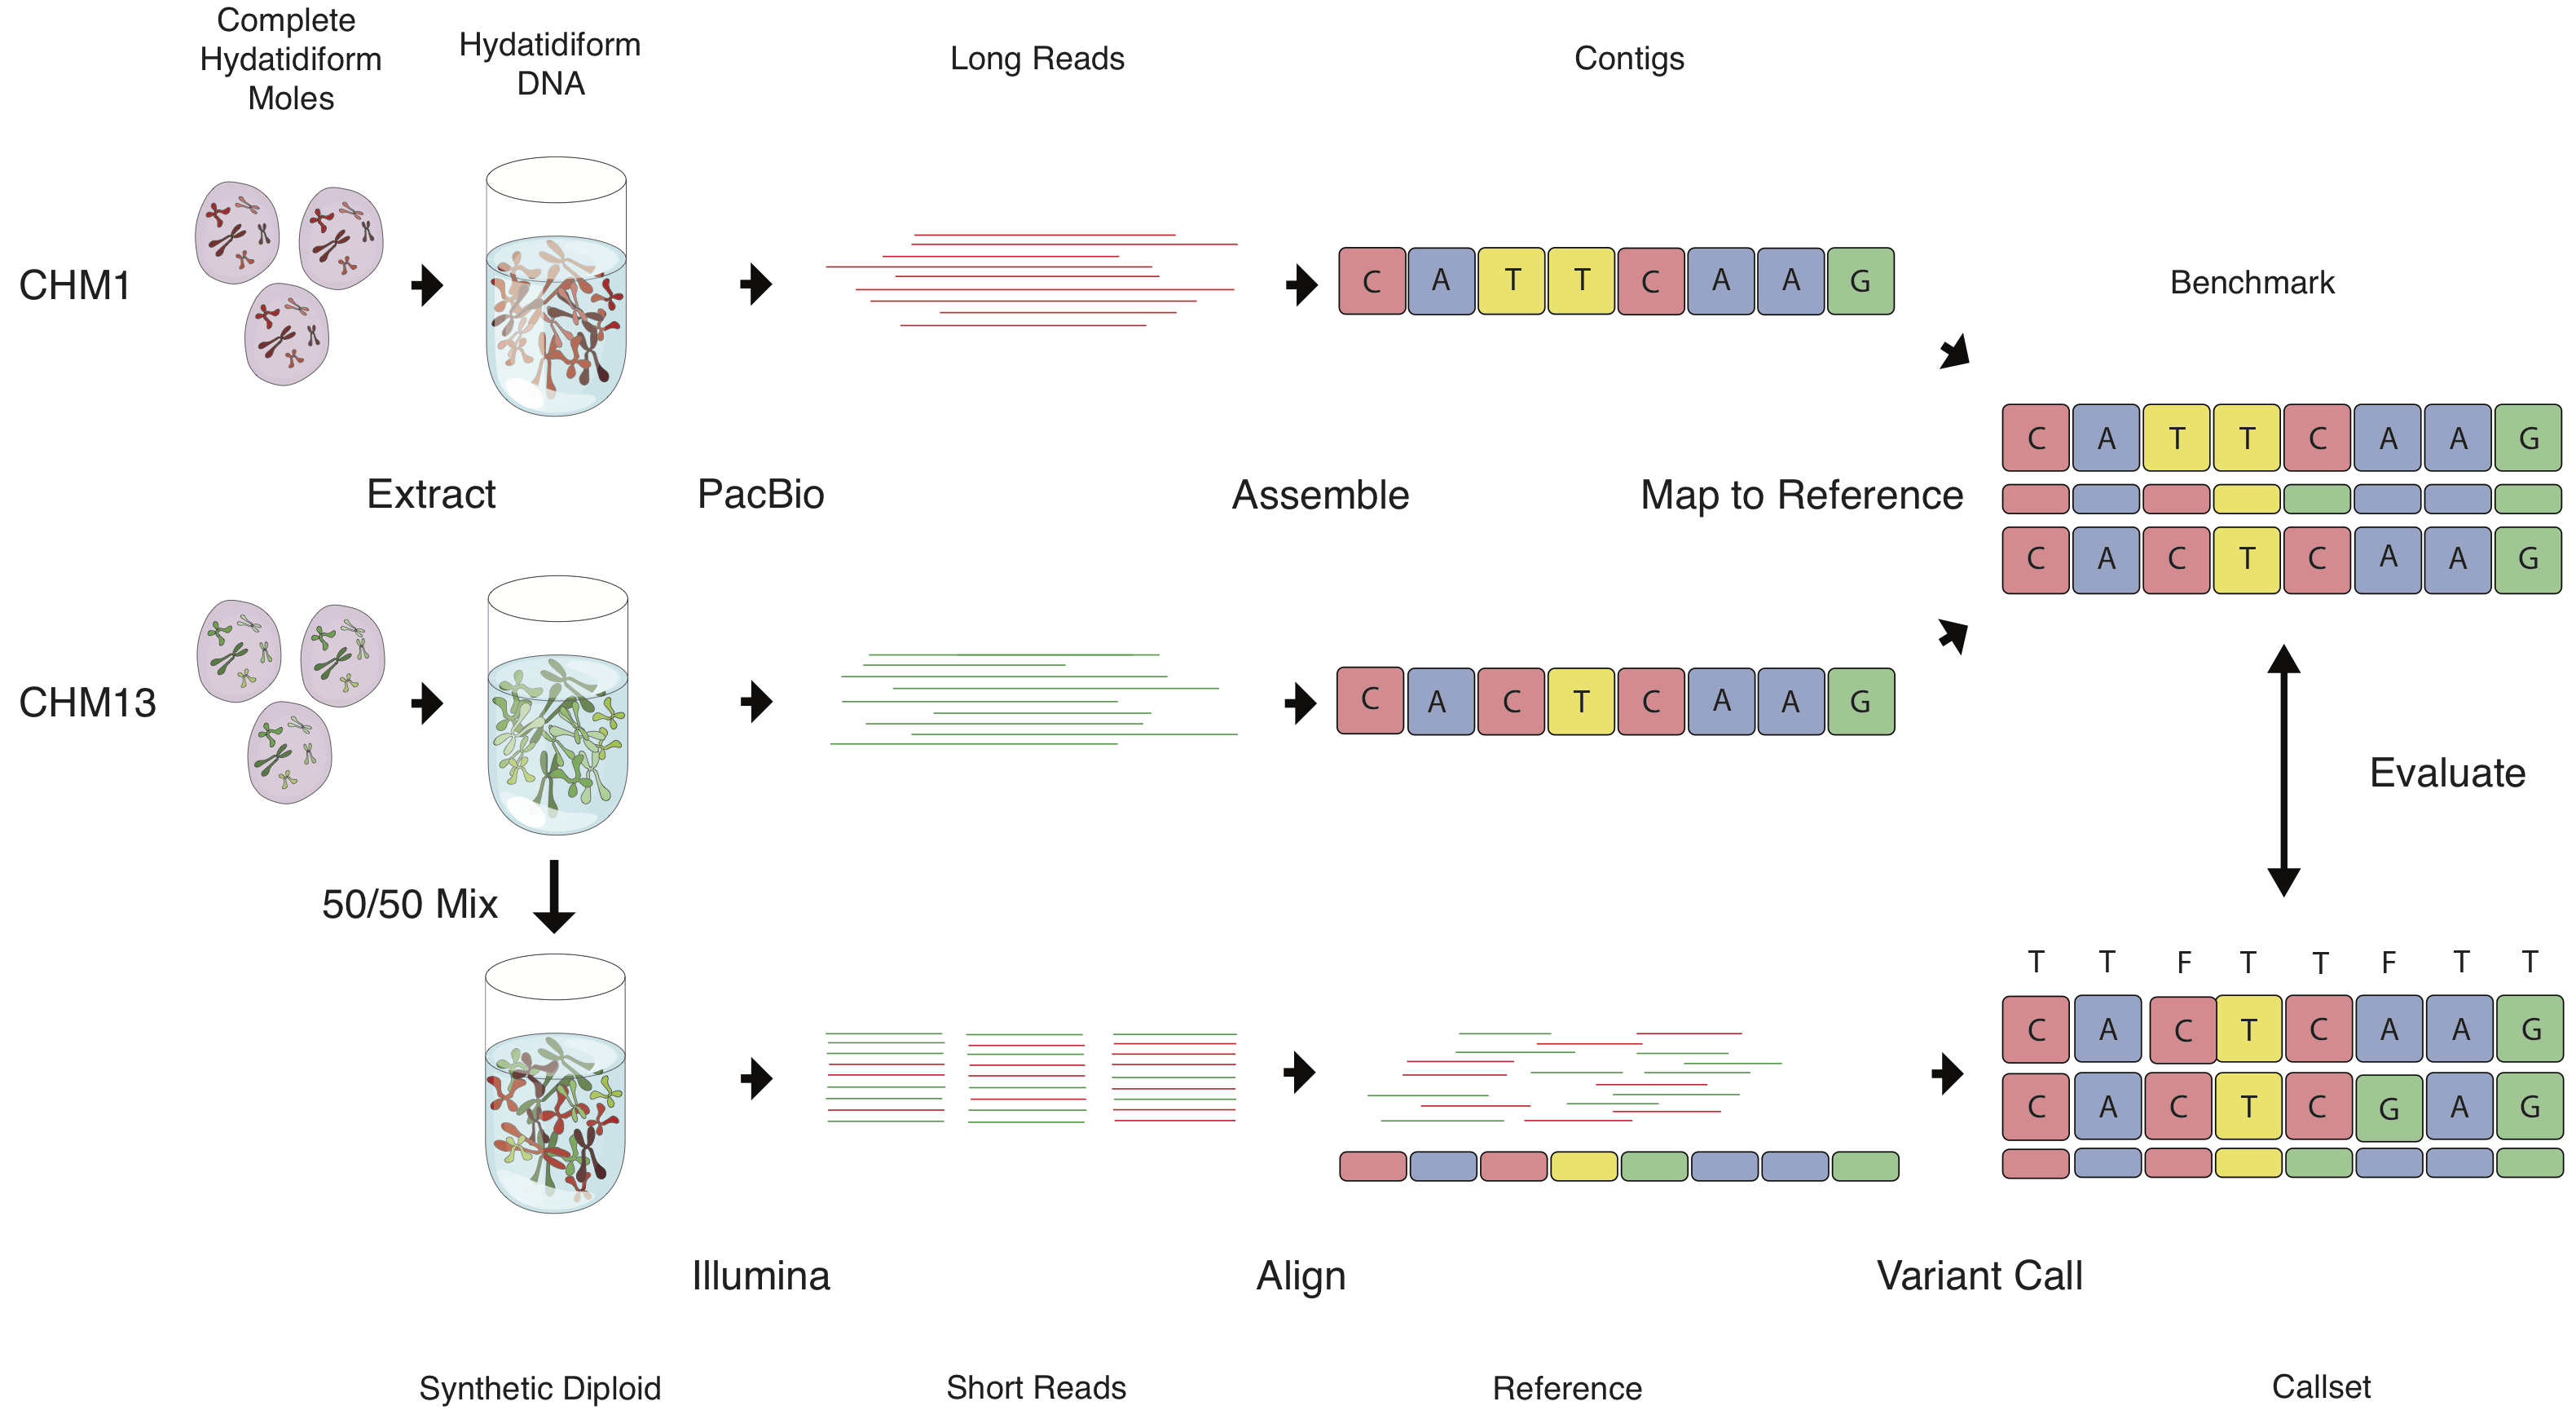
\includegraphics[width=.49\textwidth]{CHM-workflow.pdf}
\caption{Constructing the Syndip benchmark dataset. CHM1 and CHM13 cell lines
were sequenced with PacBio and \emph{de novo} assembled
independently~\citep{Schneider:2017aa}. Assembly contigs were aligned to the
human reference genome. Differences in the alignment were taken as `true' SNPs
and INDELs; regions covered by exactly one contig from each CHM assembly were
identified as confident regions where true variants can be called to high
accuracy. For the evaluation of diploid variant calling with short reads, the
same amount of DNA from the two cell lines were experimentally mixed. A
PCR-free library was constructed from the mix and sequenced to $\sim$40-fold
coverage with 151bp paired-end reads.  Variants called from the short reads
were compared to the PacBio variants to measure accuracy.}\label{fig:flow}

\end{figure}

The resulting benchmark dataset is Syndip (synthetic diploid;
Fig.~\ref{fig:flow}). We excluded 1bp INDELs as the PacBio error rate of these
INDELs is higher, especially around poly-C homopolymer runs. We also excluded
poly-A runs $\ge$10bp in length for a similar reason. In the end, we generated
3.53 million SNPs and 0.38 million 2--50bp INDELs, in 2.70 gigabases (Gbp) of
confident regions, covering 95.4\% of autosomes and X chromosome of GRCh37.

We experiementally mixed DNA from the two CHM cell lines to 50-50 percent and
sequenced with Illumina HiSeq X Ten (Fig.~\ref{fig:flow}). By counting supporting
reads at heterozygous SNPs after variant calling, we estimated 50.7\% of DNA in
the mixture comes from one cell line and 49.3\% from the other. The mixture is
a good representative of a diploid sample. We mapped the reads from the
pseudo-diploid samples to the human genome with BWA-MEM-0.7.15~\citep{Li:2013aa},
Bowtie2-2.2.2~\citep{Langmead:2012fk}, minimap2~\citep{Li:2017kk} and SNAP-0.15.7~\citep{Bolosky:2014aa}, and called variants on the pseudo-diploid
samples with FermiKit-0.1.13~\citep{Li:2015eu},
FreeBayes-1.0.2~\citep{Garrison:2012aa}, Platypus-0.8.1~\citep{Rimmer:2014ab},
Samtools-1.3~\citep{Li:2011ab} and GATK-3.5~\citep{Depristo:2011vn}, including
the HaplotypeCaller (HC) and UnifiedGenotyper (UG) algorithms. We included
multiple variant callers to avoid overemphasizing caller-specific
effects.

\begin{figure*}[!tb]

\includegraphics[width=\textwidth]{fig1.pdf}
\caption{Percent false negative rate (\%FNR) and number of false positives per
million bases (FPPM) of different variant calling algorithms.  For two variant
call sets $A$ and $B$, a call in $A$ is said to be \emph{found} in $B$ if there
is a call in $B$ that is within 10bp around the call in $A$. Given a truth and
a test call set, a \emph{true positive} (TP) is a true variant also found in
the test call set; a \emph{false negative} (FN) is a true variant not found in
the test call set; a \emph{false positive} (FP) is a test variant call not
found in the truth call set.  \%FNR=100$\times$FN/(TP+FN);
FPPM=\mbox{$10^6\times$ FP/$L$}, where $L$ is the total length of confident
regions.  Variants not overlapping confident regions, 1bp INDELs and $>$50bp
INDELs are not counted as TP, FN or FP. For `FreeBayes*', alignments with five
or more mismatches of base quality 20 or higher were dropped before FreeBayes
was applied.  (a) comparison of Syndip, GIAB and PlatGen benchmark data sets
on filtered calls. For GIAB and PlatGen, variants were called from the HiSeq X
Ten run `NA12878\_L7\_S7' available from the Illumina BaseSpace. (b) effect of
composite variant filters: variant quality $\ge$30; read depth at the variant below
$d+4\sqrt{d}$ with $d$ being the average read depth; the fraction of variant
supporting reads $\ge$30\% of total read depth at the variant (25\% for
FermiKit); Fisher strand P-value $\ge0.001$; the variant allele is
supported by at least one read from either strand. (c) effect of genomic
regions.  Low-complexity regions were identified with the symmetric DUST
algorithm~\citep{Morgulis:2006aa} at a score threshold 30. The `hard-to-call' regions include
low-complexity regions, regions unmappable with 75bp single-end reads and
regions susceptible to common copy number variations~\citep{Mallick:2016aa}. Panel (d)--(f) are
only showing metrics in `coding+conserved' regions. (d) effect of the human
genome build. Decoy sequences were identified by the 1000 Genomes project. They
are supposedly real human sequences that are missing from GRCh37.  (e) effect
of the mapping algorithms and post-processing. Red bar runs BWA-MEM and applies
base quality recalibration (BQSR) and INDEL realignment (Realn). INDEL accuracy
on SNAP alignment is only shown for GATK-HC because
others do not work well with not edit-based SNAP alignments. (f) effect of
replicates.  Replicate 1--4 were sequenced from a library consisting of DNA
from both CHM cell lines prior to library construction; Replicate 5* was
generated by computationally subsampling and mixing reads sequenced from the
two CHM cell lines separately.  Replicate 1 is used in panel
(a)--(e).}\label{fig:fig1}

\end{figure*}

In Figure~\ref{fig:fig1}, we evaluated variant calling pipelines on different
conditions. We measured the accuracy with two metrics: the percent false
negative rate (\%FNR) and the number of false positive calls per million bases
(FPPM), which equals the false positive rate scaled by $10^6$. In comparison to
the more popular metric precision [=TP/(TP+FN)], FPPM does not depend on the
rate of variations and is thus more comparable across data sets of different
populations or species. Figure~\ref{fig:fig1}a reveals that the FPPM of SNPs
estimated from Syndip is often 5--10 times higher than FPPM estimated from
GIAB or PlatGen.  Looking into the Syndip false positive (FP) SNPs, we found
most of them are located in potential CNVs that are evident in PacBio data in
the context of long flanking regions, but look dubious in short-read data
alone. GIAB-3.3.1 and PlatGen-1.0 often exclude these false positives from the truth set
based on the pedigree information or orthogonal data.  However, in real
applications, we often only have access to Illumina data and thus cannot
achieve the accuracy suggested by the two benchmark data sets.

In evaluation, we used filtered variant calls instead of raw calls. For
GATK-HC, filtering only reduces sensitivity by 1\%, but reduces the number of FPs by
five folds (Figure~\ref{fig:fig1}b), reduces the number of coding SNPs absent
from the 1000 Genomes Project~\citep{1000-Genomes-Project-Consortium:2015aa} by
58\%, and reduces the number of loss-of-function (LoF) calls by 30\%. We
manually inspected 20 filtered LoF calls in
IGV~\citep{Robinson:2011uo}. All of them are either false positives or outside
confident regions; those outside confident regions do not look real, either.
False positives are enriched among LoF calls because real LoF mutations are
subjected to strong selection but errors are not. For functional analyses, such
as in the study of Mendelian diseases, we strongly recommend to apply stringent
filtering to avoid variant calling artifacts. We note that the popular metric
F1-score, which is the average of sensitivity [=TP/(TP+FP)] and precision, is usually higher for unfiltered calls. For example, on GIAB,
the F1-score of unfiltered GATK-HC SNP calls is 0.998, higher than that of
filtered calls 0.991. It may not reflect the accuracy important to clinical
applications.

Consistent with our previous finding~\citep{Li:2014ac}, most FP INDELs come
from low-complexity regions (LCRs), 2.3\% of human genome
(Figure~\ref{fig:fig1}c). While this finding helps to guide our future
development, it over-emphasizes a class of INDELs that often have unknown
functional implications. To put the evaluation in a more practical context,
we compiled a list of potentially functional regions, which consist of coding
regions with 20bp flanking regions, regions conserved in vertebrate or
mammalian evolution and variants in the ClinVar or GWAScatalog databases with
100bp flanking. Only 0.5\% of regions intersect with LCRs. As a result, the
FPPM of INDELs in these regions is much lower.

We found mapping reads to GRCh38 leads to slightly better results than mapping
to GRCh37 alone (Figure~\ref{fig:fig1}d), potentially due to the higher quality
of the latest build. Although mapping to GRCh37 with decoy sequences further
helps to reduce FP calls, this often comes at a minor loss in sensitivity.
The choice of read mapping pipelines affects variant calling accuracy more
(Figure~\ref{fig:fig1}e). Bowtie2 alignment often yields lower FPPM because
Bowtie2 intentionally lowers mapping quality of reads with excessive
mismatches, which helps to avoid FPs caused by divergent CNVs.  We tried a
similar heuristic in the `FreeBayes*' method by discarding alignments with
excessive high-quality mismatch bases prior to variant calling. It indeeds
improves FPPM as well.  However, downweighing such alignments may lead to a
bias against regions under balancing selection or reduce sensitivity for
species with high heterozygosity. It might be preferred to implement such a
filter as a post-alignment or post-variant filter. We observed comparable
FPPM but varying sensitivity across four biological replicates
(Figure~\ref{fig:fig1}f). Replicate 4 has the lowest coverage and base quality.
The variant calling sensitivity is also the lowest. Importantly,
Figure~\ref{fig:fig1}f suggests computationally subsampling and mixing reads
sequenced from each CHM cell line separately, which is technically easier than
experimental DNA mixing to precise fraction, may be adequate to the evaluation
of short variant calling.

We have manually inspected FPs and FNs called by each variant caller. GATK-HC
performs local re-assembly. It consistently achieves the highest INDEL
sensitivity.  However, it may assemble a wrong haplotype around a long INDEL in
a long LCR and make a false INDEL call distant from the truth INDEL. We believe
this can be improved with a better assembly algorithm as FermiKit, which also
performs assembly, is less affected.  FreeBayes is efficient and very good at
SNP calling. A caveat is that it does not penalize reads with intermediate
mapping quality as much as other variant callers, which may lead to high
FPPM in regions affected by CNVs.  For single-sample variant calling on
BWA-MEM alignments, we recommend to filter alignments with excessive
high-quality mismatches. This improves FPPM with little loss in sensitivity.
Platypus and SAMtools are also competent variant callers. Nonetheless, they may
call the same INDEL twice at different places even if at the wrong place there
are only a couple of reads directly supporting the INDEL. This affects their
FPPM.  It is not obvious how to filter such false INDELs without looking at the
underlying alignments.

Syndip is a special benchmark data set that can only be constructed when
high-quality PacBio assemblies of two independent homozygous cell lines are
available at the same time. It draws the power of long-read sequencing
technologies while avoiding the difficulties in calling heterozygotes from
relatively noisy data. Syndip is the first benchmark data set that does not
heavily depend on short-read data and short-read variant callers, and thus more
honestly reflects the true accuracy of variant callers. On the other hand,
Syndip also has weakness. The PacBio consensus of homozygous genomes
is still associated with a small error rate. Errors in the consensus may appear
to be false negatives of short-read call sets. We excluded 1bp INDELs and
INDELs in long poly-A runs to alleviate this problem but lost the ability to
evaluate such INDELs in the mean time. In addition, due to misassemblies in
PacBio data and the difficulties in interpreting SVs, Syndip does not cover
the entire genome. It is still biased towards relatively easy genomic
regions. Better PacBio assembly and long-read based SV calling may further
improve the Syndip benchmark data set.

\paragraph{Data availability\textcolon} Illumina reads from this study were
deposited to ENA under accession PRJEB13208. This includes one run for each CHM
cell line and four runs for experimental mixtures. Syndip
variant calls, confident regions and evaluation script can be downloaded from
https://github.com/lh3/CHM-eval.

%\section*{Acknowledgements}
%
%(funding)

\bibliography{CHM}

\begin{methods}

\section*{Methods}\label{sec:methods}

\subsubsection*{Identifying misassembled regions on PacBio contigs}

We acquired CHM1 and CHM13 \emph{de novo} assemblies (accession GCA\_001297185
and GCA\_000983455, respectively) from NCBI and downloaded Illumina short reads
from SRA (accession SRR2842672 and SRR3099549 for CHM1; SRR2088062 and
SRR2088063 for CHM13). We assembled Illumina data with FermiKit, mapped
to the corresponding PacBio assemblies and called 60,682 heterozygous
substitutions from CHM1 and 187,267 from CHM13. These heterozygous substitutions
are often close to each other and have higher-than-average Illumina read depth.
They are probably due to misassemblies in the PacBio assembly. We
hierarchically clustered heterozygous events as follows: we merged two clusters
adjacent on the PacBio assembly if 1) the minimal distance between them is with
10kb and 2) the density of heterozygotes in the merged cluster is at least 1
per 1kb. We identified about 3,000 clusters containing three or more
heterozygotes from each PacBio assembly, and softly masked these clustered
regions to avoid them complicating downstream variant calling.
%About 10,000 heterozygous substitutions from each genome are still unmasked at this step. 

\subsubsection*{Constructing the truth call set and confident regions}

For each CHM PacBio assembly, we split the contigs into 200kb subsequences
without overlaps and mapped the split sequences to GRCh37 with BWA-MEM with the
`-x intractg' option. To call pseudo-diploid variants from PacBio assemblies,
we merged the assembly-to-reference alignments of CHM1 and CHM13. We discarded
alignments with mapping quality below 20, dropped aligned segments shorter than
10kb and made an unfiltered call set by reading the differences between the
PacBio contig and GRCh37.

We constructed the initial set of confident regions from the same alignment.
For each PacBio assembly, we say a region on GRCh37 is \emph{orthologous} to
the assembly if 1) the region is covered by one PacBio alignment longer than
10kb with mapping quality no less than 20; 2) the region is not covered by
another PacBio alignment longer than 1kb, regardless of the mapping quality; 3)
the aligned position on the PacBio contig is not in a misassembled region
identified previously. The initial set of confident regions is the intersection
of GRCh37 regions orthologous to both CHM1 and CHM13. These regions cover
96.2\% of GRCh37.

In downstream evaluation, we later noticed that if a small region harbors many
variants, the region tends to be enriched with errors potentially due to
misalignments or structural variations.  We thus applied another hierarchical
clustering to spot clusters of variations.  More precisely, in this clustering
procedure, we merged two clusters if 1) the minimal distance between two
variants is with 250bp and 2) the density of variants in the merged cluster is
at least 1 per 50bp. We collected clusters consisting of 10 or more variants
and excluded the related regions from the initial confident regions. The final
confident regions cover 95.9\% of GRCh37, or 95.4\% if we exclude poly-A runs
$\ge$10bp. We also applied a similar procedure to GRCh37 with decoy contigs and
to GRCh38.

To confirm the quality of the Syndip data set, we manually inspected several
hundred differences in IGV~\citep{Robinson:2011uo}. We observed that 10--20\%
of false positive and false negative INDEL calls made by HaplotypeCaller appear
to have strong support from Illumina reads. Most of them are around
low-complexity regions (LCRs) and supported by both Illumina reads sequenced by
us and Illumina reads downloaded from SRA. We speculate that the
PacBio-Illumina differences are enriched with consensus errors in PacBio
contigs, though somatic mutations and systematic Illumina errors may also
contribute. Anyway, even if Illumina data were all correct, 10--20\% would not
change our general conclusions or the relative performance between calling
methods as PacBio contig errors or somatic mutations are not biased towards a
particular calling method.

\subsubsection*{Calling SNPs and short INDELs from Illumina data}

We mapped the reads to the human genome GRCh37 with the GATK best-practice
pipeline, which uses BWA-MEM for mapping and post-processes alignments with
BQSR and INDEL realignment, and mapped the reads from one sample with BWA-MEM
to various human genome versions without post processing steps. We have also
run Bowtie2, minimap2 and SNAP for the same sample. We used the default
settings of various mappers, except for tuning the maximal insert size.

We called variants on the pseudo-diploid samples with FermiKit, FreeBayes,
Platypus, Samtools and GATK, including the HaplotypeCaller (HC) and
UnifiedGenotyper (UG) algorithms and filtered the raw variant calls with a set
of rules described in the caption of Figure~\ref{fig:fig1}.  We have tried
GATK's VQSR model for filtering. However, as the VQSR training set is biased
towards variants in highly unique regions, VQSR misses many truth variants
without perfect averaged mapping quality. Both GATK and Platypus come with a
set of hard filters. However, not setting filters on read depth, one of the
most effective filters on single-sample calling, these filters lead to a low
precision.

We have tried a similar heuristic used for the `FreeBayes*' method by lowering
the mapping quality of alignments with excessive high-quality mismatches down
to zero. This heuristic reduces the INDEL FPPM of GATK-HC from 1.1 to 0.7, but
increases \%FNR from 7.3 to 10.6. Similar magnitude is observed for GATK-UG,
Platypus and SAMtools. In comparison, this heuristic only affects FreeBayes
\%FNR by 0.2\%. We felt the loss of INDEL sensitivity unacceptable, so did not
apply it to GATK-HC and other callers.

The variant calling pipeline and filters have been implemented in
https://github.com/lh3/unicall.

\end{methods}

\end{document}
